%!TEX root=../document.tex
\section{Architektur - A09 Server-Client-Chat}
	\subsection{Aufgabenstellung}
	Verwende das Decorator Pattern, um die Socket-Kommunikation zwischen einem einfachen Server und einem simplen Client (Konsole genügt) zu dekorieren! Die Plaintext-Kommunikation kann z.B. mit einer RSA- oder AES-Verschlüsselung, einer BASE64-Codierung, einem Hashwert / Fingerprint dekoriert werden.
	
	Zeige im Code, dass die unterschiedlichen Dekorierer miteinander kombiniert werden können!
	
	\subsection{Umsetzung}
	Für die Umsetzung wurde wie vorausgesetzt ein Decorator Pattern verwendet.
	Hierbei wird ein angepasster Stream dekoriert. Dieser wird mit einem Socket ausgestattet und dekoriert somit immer die \texttt{write} bzw. die \texttt{read} Methode.
	
	Somit kann bsp. ein \texttt{AESDecorator} erstellt werden, welcher in der \texttt{write} Methode mithilfe eines \textit{Block - Ciphers} den Text verschlüsselt und anschließend in der zugehörigen \textit{read} Methode wieder entschlüsselt.
	
		\subsubsection{UML - Klassendiagramm}
		Das Decorator Pattern wurde nach folgender Struktur umgesetzt.
		\vspace{0.2cm}
		\begin{figure}[!h]
			\begin{center}
				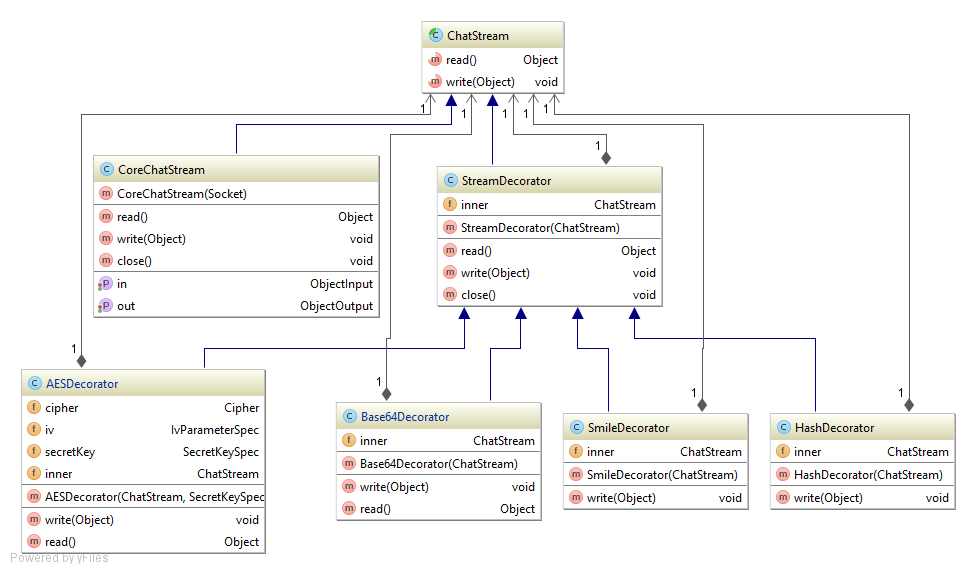
\includegraphics[width=0.76\linewidth]{images/decdiagram.png}
			\end{center}
		\end{figure}
		
			\paragraph{\textit{ChatStream} - Komponente}\mbox{}
			\vspace{0.15cm}\\
			Zu dekorierende Komponente.\\
			Hier wird eine abstrakte Komponente als dekorierende Klasse verwendet, da ein spezielles Interface implementiert werden muss. Die Komponente bietet zwei abstrakte Methoden welche dekoriert werden.
			\begin{itemize}
				\item \textbf{\texttt{public Object read()}}\\
				Daten von dem \textit{ObjectInputStream} lesen und dementsprechend an den Aufrufer zurückliefern. 
				
				\item \textbf{\texttt{public void write(Object o)}}\\
				Ein bestimmtes Objekt mithilfe des \textit{ObjectOutputStream} schreiben.
			\end{itemize}
			
			\paragraph{\textit{CoreChatStream} - Konkrete Komponente}\mbox{}
			\vspace{0.15cm}\\
			Konkrete Implementierung des \textit{ChatStreams} / Komponente.\\
			Diese Klasse extended von der zu dekorierenden Komponente und muss aufgrund der abstrakten Methoden diese auch überschreiben und mit Funktionalität füllen.
			Wie der Name schon beschreibt ist dies die nötigste Grundfunktionalität. In diesem Fall wird ausschließlich ein \textit{Object} gelesen bzw. mit \texttt{read} geschrieben.
			
			\begin{lstlisting}[style=JavaG, caption={Konstruktor and in / out Stream CoreChatStream}]
private ObjectOutput out;
private ObjectInput in;

/**
* {@link CoreChatStream} Constructor
*
* @param socket
* @throws IOException
*/
public CoreChatStream(Socket socket) throws IOException {
	this.out = new ObjectOutputStream(socket.getOutputStream());
	this.in = new ObjectInputStream(socket.getInputStream());
}
			\end{lstlisting}
			
			\begin{minipage}{.5\textwidth}
				\begin{lstlisting}[style=JavaL, caption={read - CoreChatStream}]
 /**
 * Read from an InputStream
 *
 * @return @{@link Object} read Object
 * @throws IOException
 */
 @Override
 public Object read() throws IOException {
	 return this.in.readObject();
 }
				\end{lstlisting}
			\end{minipage}%
			\begin{minipage}{.5\textwidth}
				\begin{lstlisting}[style=JavaR, caption={write - CoreChatStream}]
/**
* Write to an OutputStream
*
* @param o @{@link Object} Object to write
* @throws IOException
*/
@Override
public void write(Object o) throws IOException {
	this.out.writeObject(o);
}
				\end{lstlisting}
			\end{minipage}
			
			\paragraph{\textit{StreamDecorator} - Decorator Komponente}\mbox{}
			\vspace{0.15cm}\\
			Diese Klasse erbt ebenfalls von der zu dekorierenden \textit{ChatStream} Klasse.\\
			Zusätzlich wird ein Attribut meist \texttt{inner} gennant, erstellt welches von dem gleichen Type wie der Decorator Komponente ist in diesem Fall \textit{ChatStream}.
			Dieses Attribut ist sozusagen der innere ChatStream. Sobald nun ein ChatStream mittels dem Decorator dekoriert wird kann mit dem Attribute \texttt{inner}, die inneren zu dekorierenden Methoden aufgerufen werden und somit rekursiv nach innen durchzuarbeiten.
			
			\begin{lstlisting}[style=JavaG, caption={Konstruktor and inner StreamDecorator}]
/**
* Inner ChatStream which will be further decorated
*/
private ChatStream inner;

/**
* {@link StreamDecorator} Constructor
* @param inner
*/
public StreamDecorator(ChatStream inner) {
	this.inner = inner;
}
			\end{lstlisting}
			
			\begin{minipage}{.5\textwidth}
				\begin{lstlisting}[style=JavaL, caption={read - StreamDecorator}]
/**
* @see ChatStream
*
* @return
* @throws IOException
*/
@Override
public Object read() throws IOException {
	return this.inner.read();
}
				\end{lstlisting}
			\end{minipage}%
			\begin{minipage}{.5\textwidth}
				\begin{lstlisting}[style=JavaR, caption={write - StreamDecorator}]
/**
* @see ChatStream
*
* @param o @{@link Object} Object to write
* @throws IOException
*/
@Override
public void write(Object o) throws IOException {
	this.inner.write(o);
}
				\end{lstlisting}
			\end{minipage}
			
			Zudem muss, nachdem der ganze ChatStream \textit{AutoClosable} implementiert, eine \texttt{close} Methode existieren, welche alle inneren Streams regelkonform schließt und auf eventuelle Fehler reagiert.
			
			\begin{lstlisting}[style=JavaG, caption={close StreamDecorator}]
/**
* Closes this resource, relinquishing any underlying resources.
* This method is invoked automatically on objects managed by the
* {@code try}-with-resources statement.
*/
@Override
public void close() throws Exception {
	this.inner.close();
}
			\end{lstlisting}
			

\clearpage


			\paragraph{\textit{AES/Base64... - Decorator} - Die Decorator Komponenten}\mbox{}
			\vspace{0.15cm}\\
			Der wichtigste Zweck dieser Klassen ist, die abstrakten Methoden in diesem Fall \texttt{read} \& \texttt{write} zu implementieren und zu ''dekorieren''.\\
			Diese Klassen erben von der DekoratorKomponente \textit{StreamDecorator} und hat somit Zugriff auf den inneren \textit{ChatStream} und somit letztendlich auf den \textit{CoreChatStream}. Somit kann das banale \texttt{read} und \texttt{write} von der \textit{CoreChatStream} Klasse erweitert oder gar komplett geändert werden.\\
			Beispiel eines Dekorators: \textit{Base64Decorator}
			
			\begin{minipage}{.5\textwidth}
				\begin{lstlisting}[style=JavaL, caption={read - Base64Decorator}]
/**
* @return
* @throws IOException
* @throws ClassNotFoundException
* @see ChatStream
*/
@Override
public Object read() throws IOException {
	Message<String> a = (Message) super.read();
	byte[] msg = a.getMessage().getBytes();
	byte[] decBytes = Base64.getDec().decode(msg);
	System.out.print("base64:" + a.getMessage());
	a.setMessage(new String(decBytes));
	return a;
}
				\end{lstlisting}
			\end{minipage}%
			\begin{minipage}{.5\textwidth}
				\begin{lstlisting}[style=JavaR, caption={write - Base64Decorator}]
/**
* @param o @{@link Object} Object to write
* @throws IOException
* @see ChatStream
*/
@Override
public void write(Object o) throws IOException {
	byte[] msg = ((Message) o).getMessage();
	byte[] encMsg = Base64.getEnc().encode(msg);
	//System.out.println("base64 encoded Message: " + new String(encodedMsg));
	Message<String> old = (Message<String>)o;
	old.setMessage(new String(encMsg));
	this.inner.write(old);
}
				\end{lstlisting}
			\end{minipage}
			
			Mithilfe des Attributs \textit{inner} kann nun auf die inneren Methoden zugegriffen werden.\\
			Das ermöglicht nun das \textbf{Decorator Pattern}. Hier wird in den Methoden \texttt{write} \& \texttt{read} ein Base64 end/dec String erzeugt und dementsprechend mit \texttt{inner/super.read} \& \texttt{inner/super.write} auf den \textit{Input/Output - Stream} geschrieben.
			
			
			\paragraph{Aufruf / Erstellen eines Stream-Decorators}\mbox{}
			\vspace{0.15cm}\\
			Hierfür ist vorallem die Reihenfolge wichtig, da ansonsten beim lesen, vor allem beim entschlüsseln und decoding Fehler auftretet können.
			
			\begin{lstlisting}[style=JavaG, caption={erstellen / Aufrufen eines Decorators}]
try (
	ChatStream stream =
		new Base64Decorator(
			new AESDecorator(
				new CoreChatStream(socket),
				skeySpec,
				iv
		)
	)
) {
			\end{lstlisting}
			
			
\clearpage


\section{Design - Patterns Allgemein}
Es gibt bereits hunderte verschiedene Design-Patterns für alle Anwendungsfälle und Programmiersprachen. Allgemein kann man jedoch den Sinn und Zweck sowie die Hintergrundgedanken als auch Vor \& Nachteile anhand dieser Beispiele gut zusammenfassen und erklären. \cite{wiki1}

Prinzipiell werden Design-Patterns verwendet um Programmcode wiederverwendbar und vor allem übersichtlich zu gestalten. Dafür gibt es zahlreiche Vorlagen und Templates. Im Prinzip gibt es zahllose Baupläne für ein passenden Software Design. Die Schwirigkeit hierbei liegt nun das \textbf{richtige} Pattern auszwählen und anzuwenden. \cite{wiki1}

Des Weiteren bieten bereits \textbf{getestete} Design-Patterns ein zuverlässiges Programmierparadigma und somit können Fehler und Gedankenfehler vorgebeugt werden. Bereits bewiesene Patterns werden mit großer Wahrscheinlichkeit auch für den eigenen Anwendungsfall genügen.

	\subsection{Klassifizierung Design-Patterns \cite{wiki1}}
	Prinzipiell können alle Arten von Design-Patterns in 3 Arten unterteilt werden.
	\begin{itemize}
		\item \textbf{Creational Patterns - [Erzeugungsmuster]}\\
		Dienen der Erzeugung von Objekten. Sie entkoppeln die Konstruktion eines Objekts von seiner Repräsentation. Die Objekterzeugung wird gekapselt und ausgelagert, um den Kontext der Objekterzeugung unabhängig von der konkreten Implementierung zu halten, gemäß der Regel: „Programmiere auf die Schnittstelle, nicht auf die Implementierung!“
		
		\item \textbf{Structural Patterns - [Strukturmuster]}\\
		Erleichtern den Entwurf von Software durch vorgefertigte Schablonen für Beziehungen zwischen Klassen. 
		
		\item \textbf{Behavioral Patterns - [Verhaltensmuster]}\\
		Modellieren komplexes Verhalten der Software und erhöhen damit die Flexibilität der Software hinsichtlich ihres Verhaltens.
	\end{itemize}
	
	Zudem kamen später noch weitere Typen für Entwurfsmuster dazu, welche zu keinen der 3 bereits genannten Typen dazu passte. Beispielsweise für Muster für Objekt rationale Abbildungen.
	Diese dienen der Ablage und dem Zugriff von Objekten und deren Beziehungen in einer relationalen Datenbank


\clearpage


	\subsection{Warum werden Deisgn-Patterns verwendet ?}
	Wie bereits angeschnitten sollen Entwurfsmuster uns dabei helfen unser Design flexibler und eleganter zu gestalten, und somit die Software wiederverwendbar machen. Aber warum sollten wir mehr Aufwand bei der Entwicklung treiben, um in der Software die eben
	genannten Eigenschaften zu realisieren?
	
	Im wesentliche verfolgt die Wiederverwendung von Software 3 wichtigen Zielen.
	
	\begin{itemize}
		\item[\Checkmark] \textbf{Reduzierung des Entwicklungsaufwandes}\\
		Da bereits die schwierige Arbeit des tüftelns getan wurde, muss das Design-Pattern lediglich noch angewendet werden.
		
		\item[\Checkmark] \textbf{Erreichung einer Qualitätsverbesserung}\\
		Da diese Patterns sich offenbar schon bewahrt haben kann man auf jeden Fall davon ausgehen, dass diese auch ''optimal'' umgesetzt sind. Zudem kommt, dass man durch diese Muster gezwungen ist, sich nach diesem Bauplan zu halten, welches selbstverständlich auch die insgesamte Qualität erhöhen kann.
		
		\item[\Checkmark] \textbf{Einheitliche Wartbarkeit}\\
		
	\end{itemize}
	

\clearpage






